\subsection{Heat Pipe problem}
\subsubsection*{Background}
When an unsaturated porous medium subjected to a constant heat flux and the temperature is sufficiently high, water is heated and vaporizes. Vapor flows under its pressure gradient towards the cooler end where it condenses. Vaporization and condensation produce a liquid saturation gradient, creating a capillary pressure gradient inside the porous medium. Condensate flows towards the hot end under the influence of a capillary pressure gradient. This is a heat pipe in an unsaturated porous medium

Udell and Fitch derived the pressure gradient of each phase in two-phase flow with heat transfer. The generalized form of the Darcy's law is used to calculate velocity fields. 
\begin{equation}
\frac{d p^g}{d x} = \frac{\eta q \nu^g}{\mathbf k k_{\mathrm {rg}} H_{\mathrm {vap}}}
\label{eq:HP1}
\end{equation}
\begin{equation}
\frac{d p^l}{d x} =- \frac{\eta q \nu^l}{\mathbf k k_{\mathrm {rl}} H_{\mathrm {vap}}}
\label{eq:HP2}
\end{equation}
where, $\eta$ is the ratio of heat transport caused by convection to the total heat-flux $q$ (see Helming [1997]). $p$ is phase pressure; $\nu^\gamma=\frac{\mu\gamma}{\rho^\gamma}$; $x$ is space coordinate in the x-direction; $\mathbf k$ is intrinsic permeability; $k_{r\gamma}$ is relative permeability and $H_{\mathrm {vap}}$ is latent heat of water. $\gamma$ is the phase superscript and $g, l$ stand for gas and liquid phase, respectively. Gas pressure is the sum of two partial pressure, i.e. $p^g=p^g_a+p^g_w$.

The density of the gas phase is the sum of air and vapor density. Air density is according to ideal gas equation,
\begin{equation}
\rho_{\mathrm {ga}}=\frac{M_a p_a}{RT} 
\label{eq:HP3}
\end{equation}
Energy transport is described by Zhou et al. [1990] as
\begin{equation}
q=-\kappa_{\mathrm {app}}\frac{\partial d T}{d x} + \dot m_{\mathrm {vap}} H_{\mathrm {vap}}
\label{eq:HP4}
\end{equation}
where, $T$ is temperature, $\kappa_{\mathrm {app}}$ is apparent thermal conductivity.

Since capillary pressure is the difference of phase pressure, hence from Eq. 1, the capillary pressure gradient is
\begin{equation}
\frac{d p^c}{d x} = \frac{\eta q}{\mathbf k H_{\mathrm {vap}}}\left[\frac{\nu^g}{k_{\mathrm {rg}}} + \frac{\nu^l}{k_{\mathrm {rl}}}\right]
\label{eq:HP5}
\end{equation}
Brooks-Corey presented a water saturation-capillary pressure relation in the following form
\begin{equation}
S=\left(\frac{Pd}{p^c}\right)^\lambda
\label{eq:HP6}
\end{equation}
By comparing this with Leverett's [1941] non-dimensional form we get $Pd=\sigma_0\left(\frac{n}{\mathbf k}\right)^{0.5}$ and $n$ is medium porosity. $\sigma_0$ is interfacial tension at reference temperature $T_0$. Here, $S$ is scaled as following 
\begin{equation}
S=\frac{S_{\mathrm {w}}-S_{\mathrm {lr}}}{1-S_{\mathrm {lr}}-S_{\mathrm {gr}}}
\label{eq:HP7}
\end{equation}
The constant $S_{\mathrm {lr}}; S_{\mathrm {gr}}$ are residual saturations. And for interfacial tension we have used following correlation given by Olivella and Gens[2000].
\begin{equation}
\sigma( T)={0.3258C^{1.256}} - {0.148C^{2.256}};~~ T\le 633.15 \mathrm K
\label{eq:surface_tension}
\end{equation}
where, $C=1.0-\frac{T}{647.3~K}$

The Brooks-Corey relative permeability relations are 
\begin{equation}
\mathbf k_{\mathrm {rg}}=\left(1-S\right)^2 \left(1-S^{\frac{2+\lambda}{\lambda}}\right);~~~\mathbf k_{rl}=S^{\frac{2+3\lambda}{\lambda}}
\label{eq:HP8}
\end{equation}
Using Eqs. (\ref{eq:HP5}-\ref{eq:HP6}), we can write following forms of saturation gradient.
\begin{equation}
\frac{d S}{d x}=\frac{S^{1.5}}{P_d}\frac{2\eta q}{\mathbf k H_{\mathrm {vap}}}\left[\frac{\nu^g}{k_{\mathrm {rg}}} + \frac{\nu^l}{k_{\mathrm {rl}}}\right]
\label{eq:HP9}
\end{equation}
Now Eq. (\ref{eq:HP9}) is integrated over two-phase zone. Where two-phase zone can be defined by imposing the limits of integration (see Udell [1985]): $S=S_0$ at $x=0$ and $S=S_1$ at $x=L$.

The saturation vapor density $\rho_{\mathrm {sat}}$, depends on temperature, and is estimated by following relation
\begin{equation}
\rho_{\mathrm {sat}}=1.0\times10^{-3}\exp\left(a-\frac{b}{T}\right)
\label{eq:HP10}
\end{equation}
where, the constants $a=19.81$ and $b=4975.9$.

In the porous medium, we must account for a decrease in vapor density due to capillarity. The amount of decrease in vapor density is describe by the Kelvin equation as follows
\begin{equation}
\rho_{\mathrm {gw}}=\rho_{\mathrm {sat}}\exp\left(-\frac{M_{\mathrm w} p^c}{\rho^l RT}\right)
\label{eq:HP11}
\end{equation}
where $M_{\mathrm w}$ is water molecular weight; $\rho^l$ is liquid density and $R$ is universal gas constant. From Eqs. (\ref{eq:HP10}-\ref{eq:HP11}), we get temperature as function of vapor density and capillary pressure as
\begin{equation}
T=\frac{A}{B}
\label{eq:HP12}
\end{equation}
where
\begin{equation*}
 A=b+\frac{M_{\mathrm w} p^c}{\rho^l R}; B=a-3 -\log\left(\rho_{\mathrm {gw}}\right)
 \label{eq:HP20}
\end{equation*}


$\rho_{\mathrm {gw}}$ is changing with temperature which introduces difficulty for the temperature calculation. Hence we need to know temperature gradient, which is possible from Eq. (\ref{eq:HP12}) along with the vapor pressure gradient 
\begin{equation}
\frac{d p_{\mathrm{gw}}}{d x} = \frac{\eta q \nu^g_w}{\mathbf k k_{\mathrm {rg}} H_{\mathrm {vap}}}
\label{eq:HP18}
\end{equation}
Form of the temperature gradient
\begin{equation}
\frac{d T}{d x}=\frac{\frac{B M_{\mathrm w}}{\rho^l R} \frac{d p^c}{d x} + \frac{A}{p_{\mathrm{gw}}} \frac{d p_{\mathrm{gw}}}{d x}}{B^2+\frac{A}{T}}
\label{eq:HP13}
\end{equation}
Apparent thermal conductivity can be obtained from heat flux divided by temperature gradient (see Udell [1985].


The coupled differential Eqs. (\ref{eq:HP1}), (\ref{eq:HP5}), (\ref{eq:HP9}) and (\ref{eq:HP13} ) are integrated using an Euler method with the following boundary conditions at $x=0$:
\begin{equation}
S=S_0;~~~ p^g=p^g_0;~~~p^c=p^c_0;~~~T=T_0
\label{eq:HP14}
\end{equation}
Material parameters are presented in Table \ref{tab:HP1}.

\subsubsection*{Definition}
The test benchmark problem for heat pipe effects is formulated in one-dimension. 
A horizontal column of length $2.6$~m is filled with fluid subjected to a constant heat flux at the right end where left end temperature maintained below to the saturation temperature.
\begin{figure}[htb]
\begin{center}
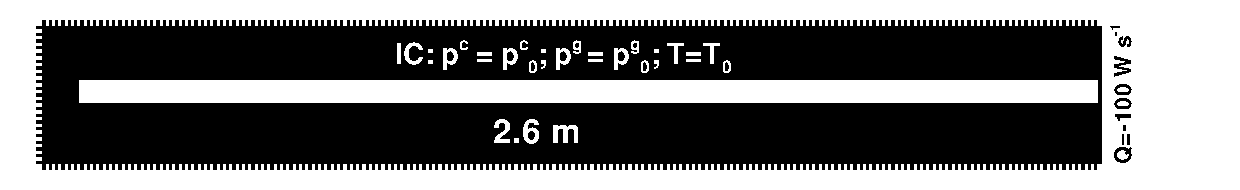
\includegraphics[height=1.25cm]{chapter_14/figures/Geo.eps}
\end{center}
\caption{Schematic of the benchmark.}
\label{Fig:HP1}
\end{figure}


\subsubsection*{Results}
In order to establish non-isothermal two-phase flow in the OpenGeoSys, we have verified numerical solutions with analytical results. Profile of water saturation $S_{\mathrm w}$, gas phase pressure $p^g$, liquid phase pressure $p^l$ and temperature $T$ are presented in Figs. \ref{Fig:HP2}, and \ref{Fig:HP4}. Numerical solutions are agreeable. Line elements have been used with variable time steps and a non uniform space discretization.
\begin{figure}[thbp]
\centerline{
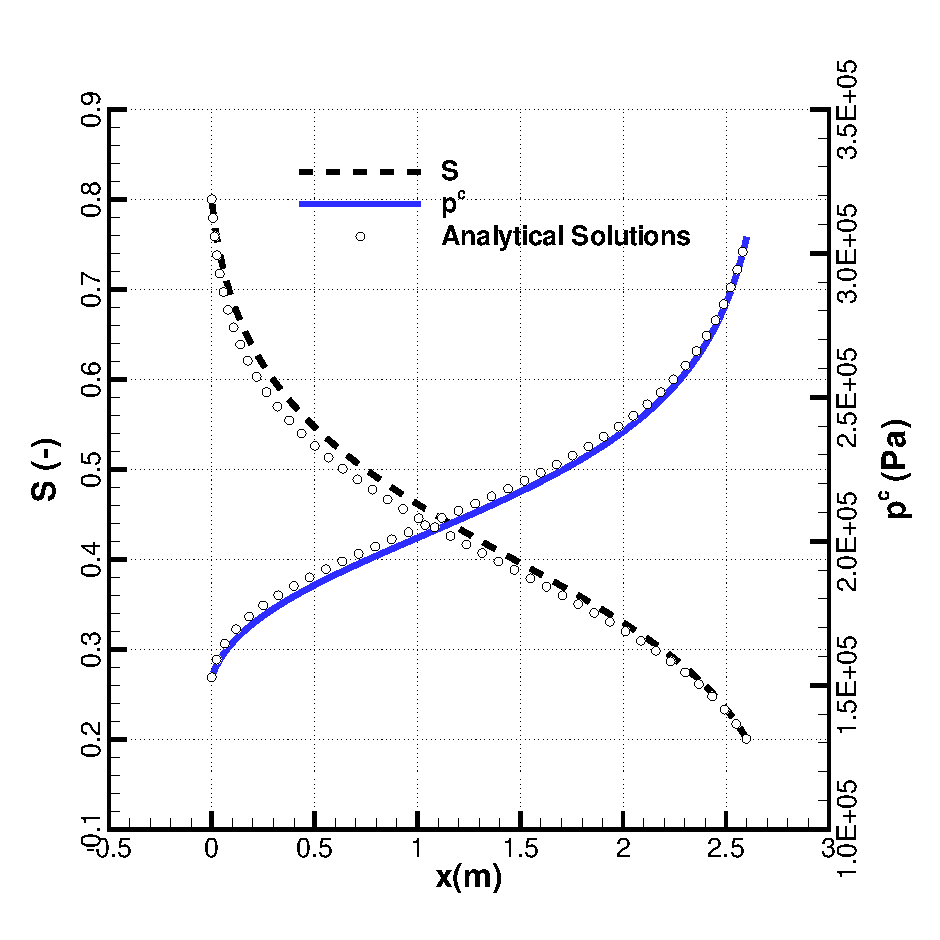
\includegraphics[height=3.0in,width=3.0in]{chapter_14/figures/S-Pc.eps}
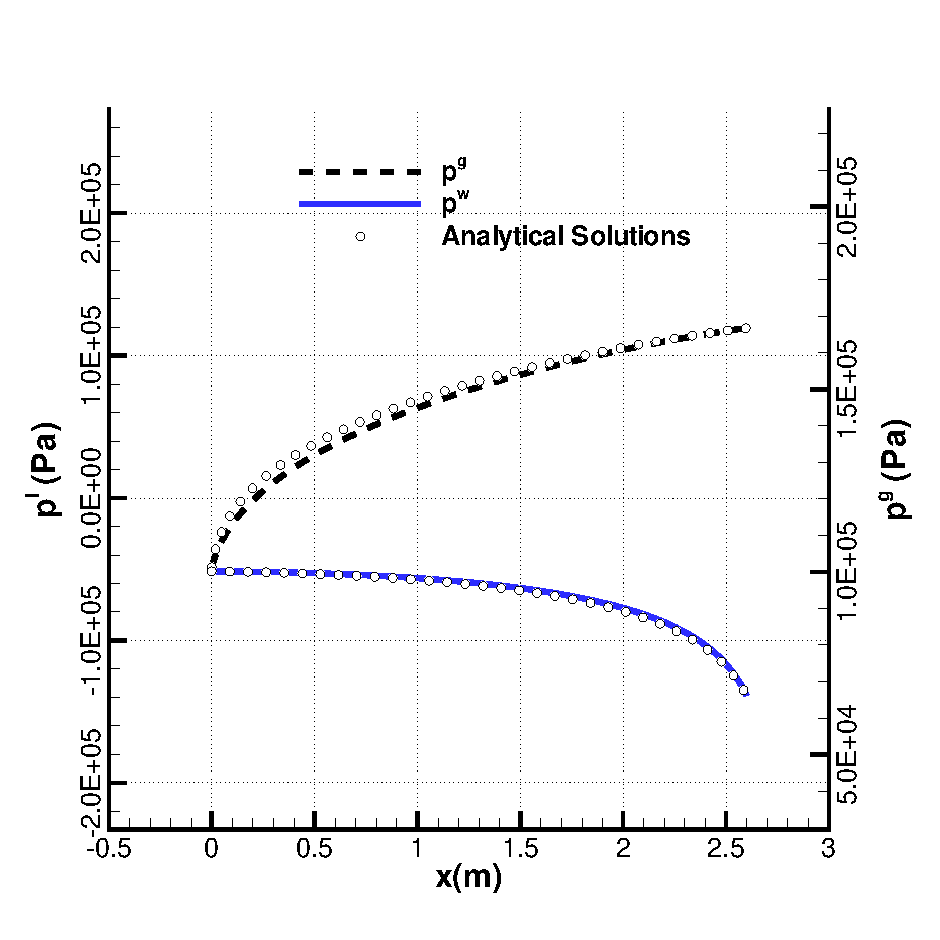
\includegraphics[height=3.0in,width=3.0in]{chapter_14/figures/Pw-Pg.eps}}
\caption{Comparison of water saturation and pressure profiles from present solution with analytical solution.}
\label{Fig:HP2}
\end{figure}
A finite element approach has been developed for the nonisothermal two-phase flow model based on the $ppT$ formulation. We used a combined monolithic/ staggered coupling scheme i.e. monolithic for the two-phase flow and staggered for the heat transport.
\begin{figure}[htb]
\begin{center}
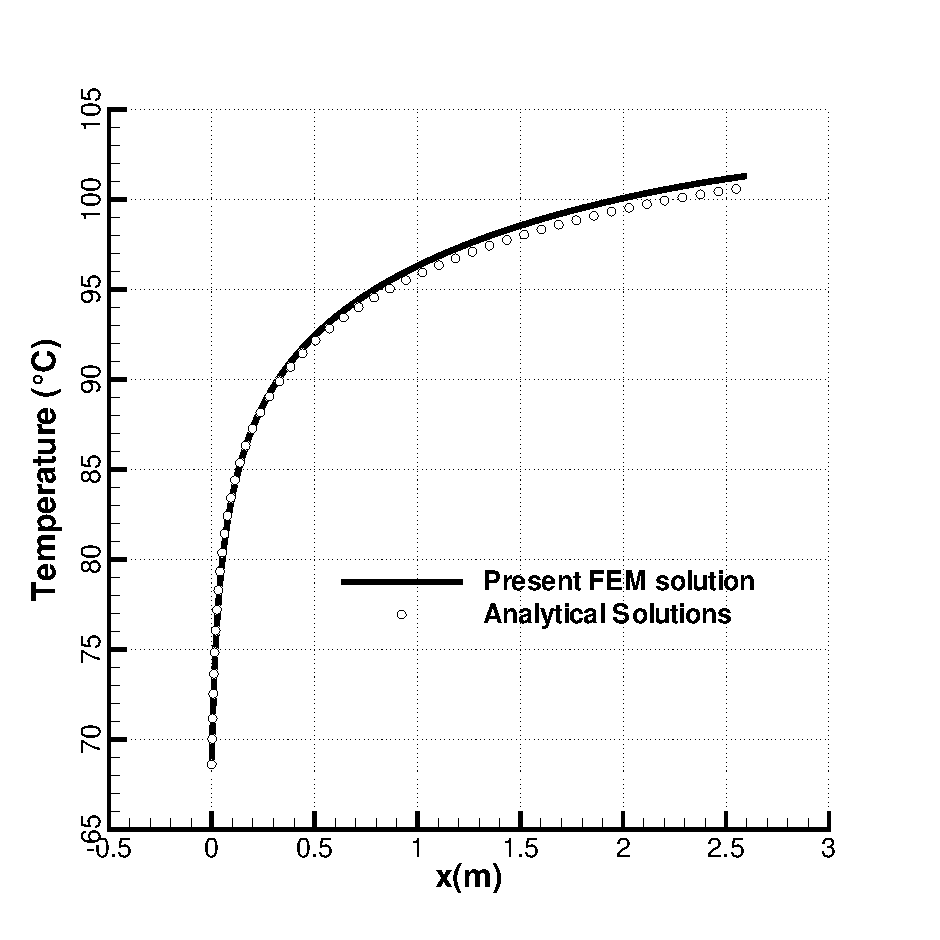
\includegraphics[height=8cm]{chapter_14/figures/Tg.eps}
\end{center}
\caption{Comparison of temperature profile from present solution with analytical solution.}
\label{Fig:HP4}
\end{figure}
\begin{table}[htbp]
\caption{Material parameters for the heat pipe problem.}
\label{tab:HP1}
\begin{tabular}{l*{4}{l}r}
\hline
\textbf{Meaning} & \textbf{Symbol} &  \textbf{Value} &  \textbf{Unit} \\
\hline
Column length & $L$ & $\mathrm m$ & $2.6$  \\
Liquid dynamic viscosity &  $\mu^l$ & $\mathrm {Pa.s}$ & $1.0\times10^{-3}$ \\
Gas dynamic viscosity & $\mu^g$ & $\mathrm {Pa.s}$ & $1.0\times10^{-5}$ \\
Liquid density &  $\rho^l$ &$\mathrm {kg.m^{-3}}$ & $1.0\times10^{3}$ \\
Permeability & $\mathbf k$ & $ \mathrm {m^2}$ & $1.0\times 10^{-13}$ \\
Porosity & $n$ & $--$ & $0.3$ \\
Residual saturation of water &  $S_{\mathrm{rl}}$ & $--$ & $0.2$ \\
Residual saturation of oil &  $S_{\mathrm{rg}}$ & $--$ & $0$ \\
Soil distribution index &  $\lambda$ & $--$ & $2.0$ \\
Capillary pressure & $p^c(S)$ & $\mathrm {Pa}$ & Brooks-Corey model\\
Relative permeability & $\kappa_{\mathrm {r\gamma}}(S)$ & $--$ & Brooks-Corey model \\ \hline
\end{tabular}
\end{table}
